\documentclass[final]{beamer}
\usepackage{type1cm}
\usepackage{calc} 
\usepackage{amsmath,amsthm, amssymb, latexsym,bm}
\usepackage{empheq}
\usepackage[english]{babel}
\usepackage[utf8]{inputenc}
\usepackage{theme} % custom
\usepackage[orientation=portrait,size=a0,scale=1.5,debug]{beamerposter}
\usepackage[absolute,overlay]{textpos}
\setbeamercolor{localBox}{bg=white}
\definecolor{mygreen}{rgb}{0,0.6,0}
\usepackage{units}
\usepackage{setspace}
\renewcommand{\rmdefault}{eulervm}
\usepackage[skins,theorems]{tcolorbox}
\definecolor{darkgreen}{rgb}{0,1.0,0}
\usepackage{mathpazo}
\usepackage{ragged2e}
\usepackage{ dsfont }
\definecolor{UniPDgray}{RGB}{72,79,89}  
\definecolor{UniPDlightgray}{RGB}{209,211,214}  
\newcommand{\RN}{RN}
\newcommand{\CH}{\text{CH}}
\newcommand{\ket}[1]{\vert{#1}\rangle}
\newcommand{\bra}[1]{\langle{#1}\vert}
\usepackage[export]{adjustbox}
\usepackage{hyperref}

%%%%%%%%%%%%%%%%%%%%%%%%%%%%%%%%%%%%%%%%%%% DOCUMENT %%%%%%%%%%%%%%%%%%%%%%%%%%%%%%%%%%%%%%%%%%%
\begin{document}
%%%%%%%%%%%%%%%%%%%%%%%%%%%%%%%%%%%%%%%%%%% HEADER %%%%%%%%%%%%%%%%%%%%%%%%%%%%%%%%%%%%%%%%%%%
\title{{Self-compensating source at 800 nm for satellite quantum key distribution}}
\vskip-0.4cm
\author{ F.~Berra, C.~Agnesi, S.~Cocchi, A.~Stanco, M.~Avesani, P.~Villoresi and G.~Vallone}
\vskip0.4cm
\institute{{\footnotesize\textbf{Department of Information Engineering, University of Padova, 35131 Padova, Italy}}}
\setlength{\TPHorizModule}{\linewidth}
\setlength{\TPVertModule}{\linewidth}

%%%%%%%%%%%%%%%%%%%%%%%%%%%%%%%%%%%%%%%%%%% BODY %%%%%%%%%%%%%%%%%%%%%%%%%%%%%%%%%%%%%%%%%%%
\begin{frame}
	%%%%%%%%%%%%%%%%%%%%%%%%%%%%%%%%%%%%%%%%%%% B1
	% \begin{textblock}{0.96}(0.03,0.168)
	% 	%\vskip 0.05cm
	% 	\justifying
	% 	{\textbf{Polarization} encoding has been extensively used
	% 		for QKD along free-space, optical fiber, and satellite links.
	% 		However, the polarization encoders used in such implementations are \textbf{unstable}, expensive, and can even
	% 		exhibit insecure \textbf{side channels}. Here we propose a \textbf{self-compensating} polarization
	% 		encoder based on a $LiNbO_3$ phase modulator inside
	% 		a \textbf{Sagnac} interferometer and implement it using only commercial off-the-shelf (COTS) components.} %Our polarization
	% 	%encoder combines a simple design and high stability reaching an intrinsic quantum bit error rate as low as $0.2\%$.
	% 	%Since realization is possible from the 800 to the 1550 nm
	% 	%band using COTS devices, our polarization modulator is a
	% 	%promising solution for free-space, fiber, and satellite-based
	% 	%QKD}
	% \end{textblock}

	%%%%%%%%%%%%%%%%%%%%%%%%%%%%%%%%%%%%%%%%%%% B2 (source 800)
	\begin{textblock}{0.96}(0.03,0.158)
		\begin{block}{\large {Free-space transmitter and receiver}}
			\vskip 0.2cm
			\begin{columns}

				%%%%%%%%%%%%%%%%%%%%%%%%%%%%%%%%%%%%%%%%%%% B2.1
				\begin{column}{0.45\TPHorizModule}
					{\textbf{Transmitter\\}}
					\vskip 0.6cm
					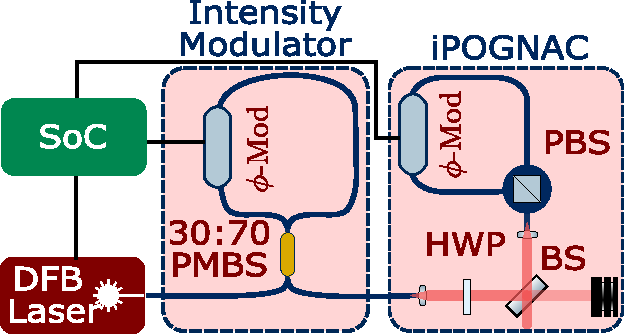
\includegraphics[scale=2.3]{imgs/trasmitter_800_nm_esa_opl.pdf}\\
					{\textbf{Features:\\}}
					\begin{itemize}
						\item \textbf{Intensity modulator}[\ref{robertz}] attenuates the pulses at single photon level $\mu_1 \approx 0.58$ and $\mu_2 \approx 0.16$
						\item \textbf{Polarization modulator}[\ref{ipognac}] generates 3-polarization states: L, R, D
						\item The source output is already in free-space excellent for satellite communications
					\end{itemize}
				\end{column}

				%%%%%%%%%%%%%%%%%%%%%%%%%%%%%%%%%%%%%%%%%%% B2.3

				\begin{column}{0.45\TPHorizModule}
					{\textbf{Receiver\\}}
					\vskip 0.6cm
					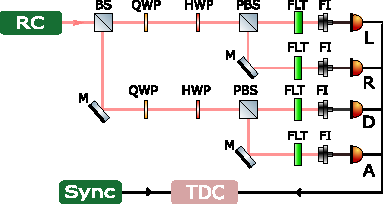
\includegraphics[scale=4]{imgs/state_analyzer_800.pdf}\\
					{\textbf{Features:\\}}
					\begin{itemize}
						\item A beam-splitter randomly projects the incoming qubits into two basis $X, Y$
						\item Each bases measures two orthogonal states $X = \{D, A\}$ and $Y = \{L, R\}$
						\item The arrival time of qubits is then synchronized with an external source for post-processing
					\end{itemize}
				\end{column}

			\end{columns}
		\end{block}
		%\vskip0.3cm
	\end{textblock}

	%%%%%%%%%%%%%%%%%%%%%%%%%%%%%%%%%%%%%%%%%%% B3 (ipognac)
	\begin{textblock}{0.965}(0.03,0.55)
		%%%%%%%%%%%%%%%%%%%%%%%%%%%%%%%%%%%%%%%%%%% B3.1
		\begin{block}{\large iPOGNAC technology }
			\vskip 0.2cm
			% \begin{flushleft}
			% 	\textbf{All the previous problems can be solved} placing a phase modulator with polarization maintaining fibers inside an asymmetric Sagnac interferometer, in a configuration similar to the intensity modulator proposed in [\ref{im}] \\
			% \end{flushleft}
			% \vskip -0.3cm
			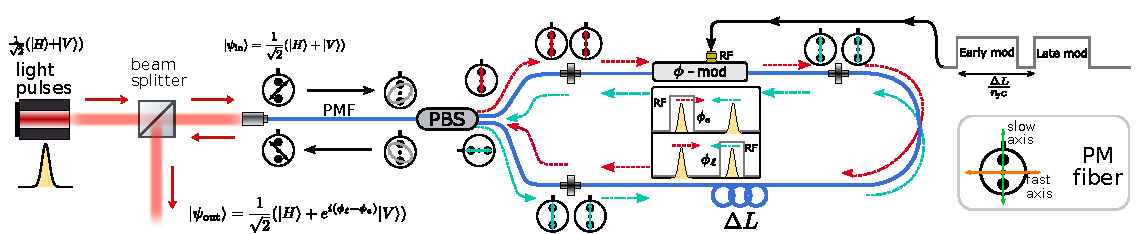
\includegraphics[scale=3.9]{imgs/ipognac.pdf} \\
			\begin{columns}

				%%%%%%%%%%%%%%%%%%%%%%%%%%%%%%%%%%%%%%%%%%% B3.2
				\begin{column}{0.46\TPHorizModule}
					%\vskip 0.02cm
					%We extract secure random numbers from the measure of the quadratures of an unknown state of the EM field (usually the vacuum). 
					\vskip -2cm
					\hskip 1cm \textbf{Features:}
					\begin{itemize}
						\item \textbf{Long term stability}: Thermal and mechanical phase drifts  are automatically compensated \\
						\item Phase modulator needs to support \textbf{only one polarization}\\
						\item \textbf{Low $V_\pi$}: no need to modulate the relative phase\\
					\end{itemize}

					\vskip1.5cm
					\textbf{\hskip1cm  Working principle: }
					\begin{itemize}
						\item The qubits enter with $\ket{D}$ state into a polarization maintaining (PM) fiber where it get an elliptical phase $\delta$  \\
						\item A fiber Polarization Beam Splitter (PBS) \textbf{splits} the light into two \textbf{orthogonal polarizations}, guided by PM fibers \\
						\item Both beams are \textbf{aligned to the slow axis} of the PM fiber. The polarization degree of freedom is mapped to the optical path of the photons. From now, \textbf{only one polarization travels in the loop}.\\
						      \vskip 0.3cm
						\item The phase modulator, placed \textbf{asymmetrically}, can add a \textbf{$\phi_e$} to the \textbf{Clockwise} pulse and a \textbf{$\phi_\ell$} shift to the \textbf{Counter-clockwise} pulse. \\

						\item At the PBS the pulses are recombined
						\item The qubits entering again in the polarization maintaining (PM) fiber with swapped $H, V$ components getting an elliptical phase $-\delta$
						\item The final state is ${\ket{\psi_\mathrm{out}}  = \frac{1}{\sqrt{2}} \left[ \ket{H} + e^{i(\phi_e-\phi_\ell)} \ket{V} \right]}$


					\end{itemize}
				\end{column}

				%%%%%%%%%%%%%%%%%%%%%%%%%%%%%%%%%%%%%%%%%%% B3.3
				\begin{column}{0.46\TPHorizModule}
					%\vskip-1cm
					\textbf{\hskip 1cm Experimental results:}\\
					\vskip 0.1cm
					\begin{itemize}
						\item Implemented at \textbf{795 nm} with only COTS components  \\
						\item Repetition rate $50$ MHz
						\item \textbf{Low QBER:} $\le \bm{1\%}$ with Si SPAD at 800nm
						      % \item Long term stability of \textbf{hours}
					\end{itemize}
					\vskip 1.5cm
						{\centering
							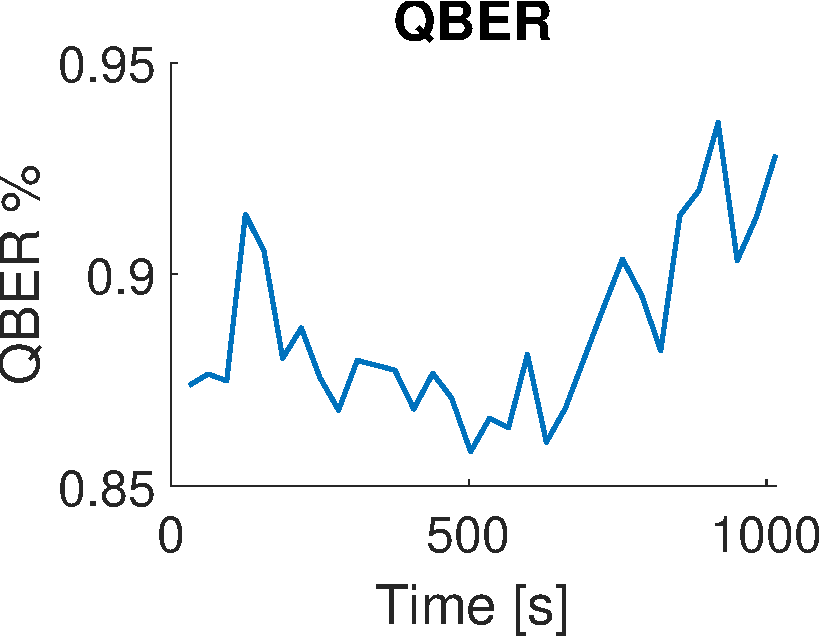
\includegraphics[width=0.4\TPHorizModule]{imgs/synchESA_fig_r5.pdf}\\
							% \includegraphics[width=0.47\TPHorizModule]{imgs/LongRun2.png}    \\
						}
				\end{column}
			\end{columns}

			%	\vskip 0.4cm
			%	\textbf{We report a generation rate of  {\large 17.39 Gbps}  of secure random numbers, certified in the Source-Device-Independent Framework.\\}
			%The setup doesn't requires active basis switching and naturally imposes a fixed bound on the $H_{min}(A|E)$}
		\end{block}
	\end{textblock}

	%%%%%%%%%%%%%%%%%%%%%%%%%%%%%%%%%%%%%%%%%%% B4 (Referencies)
	\begin{textblock}{0.965}(0.03,1.22)
		\begin{block}{\large References}
			\vskip-0.2cm
			{\footnotesize
			\begin{enumerate}
				\item G. Roberts \textit{et al.} \emph{Patterning-effect mitigating intensity modulator for secure decoy-state quantum key distribution}, Opt. Lett. \textbf{43} (20), 5110 (2018).\label{robertz}
				\item M. Avesani \textit{et al.} \emph{Stable, low-error, and calibration-free polarization encoder for free-space quantum communication}, Opt. Lett. \textbf{45} (17), 4706 (2020).\label{ipognac}
			\end{enumerate}
			}
		\end{block}
	\end{textblock}

	%%%%%%%%%%%%%%%%%%%%%%%%%%%%%%%%%%%%%%%%%%% FOOTER %%%%%%%%%%%%%%%%%%%%%%%%%%%%%%%%%%%%%%%%%%%
	\begin{textblock}{0.42}(0.6,1.4)
		\RaggedLeft {
			\color{white}
			\Large
			\textbf{federico.berra@phd.unipd.it}\\
			\textbf{https://quantumfuture.dei.unipd.it}}
	\end{textblock}
	\begin{textblock}{0.2}(0.03,1.4)
		{\color{white} \itshape \footnotesize QUANGO project:\\ EU grant agreement No. 101004341}
	\end{textblock}
\end{frame}
\end{document}


